\documentclass{article}
\usepackage{amsmath}
\usepackage{amssymb}
\usepackage{geometry}
\usepackage{tikz}
\geometry{a4paper, margin=1in}

\title{APM1220: FA 2 Solutions}
\author{}
\date{}

\begin{document}
\maketitle

\section*{Problem 3.1}
Given:
\[
X = \begin{bmatrix} 9 & 1 \\ 5 & 3 \\ 1 & 2 \end{bmatrix}
\]

\noindent \textbf{(a)} Scatter plot and sample mean \\
First, calculate the sample mean $\bar{x} = [\bar{x}_1, \bar{x}_2]'$:
\[
\bar{x}_1 = \frac{9 + 5 + 1}{3} = \frac{15}{3} = 5
\]
\[
\bar{x}_2 = \frac{1 + 3 + 2}{3} = \frac{6}{3} = 2
\]
The sample mean is $\bar{x} = \begin{bmatrix} 5 \\ 2 \end{bmatrix}$.

\begin{center}
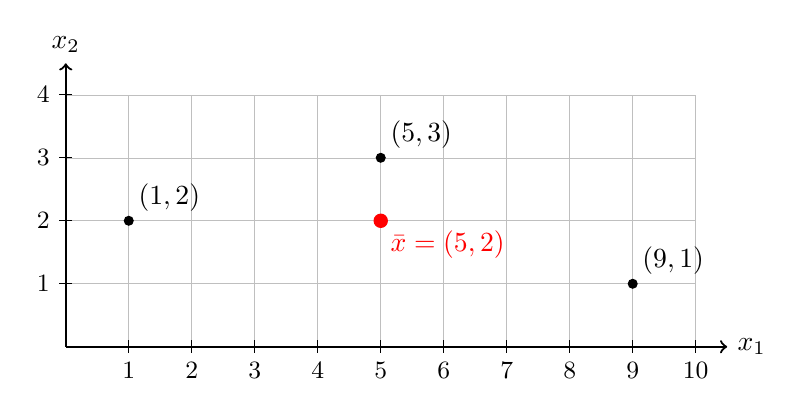
\begin{tikzpicture}[scale=0.8]
    % Grid and axes
    \draw[lightgray, very thin, step=1] (0,0) grid (10,4);
    \draw[->, thick] (0,0) -- (10.5,0) node[right] {$x_1$};
    \draw[->, thick] (0,0) -- (0,4.5) node[above] {$x_2$};
    
    % Ticks
    \foreach \x in {1,...,10} \draw (\x, 0.1) -- (\x, -0.1) node[below] {\small \x};
    \foreach \y in {1,...,4} \draw (0.1, \y) -- (-0.1, \y) node[left] {\small \y};
    
    % Points
    \filldraw[black] (9,1) circle (2pt) node[above right] {$(9,1)$};
    \filldraw[black] (5,3) circle (2pt) node[above right] {$(5,3)$};
    \filldraw[black] (1,2) circle (2pt) node[above right] {$(1,2)$};
    
    % Mean
    \filldraw[red] (5,2) circle (3pt) node[below right, red] {$\bar{x} = (5,2)$};
\end{tikzpicture}
\end{center}

\noindent \textbf{(b)} Sketch the $n=3$ dimensional representation and deviation vectors \\
Calculate the deviation vectors $d_1 = y_1 - \bar{x}_1 1$ and $d_2 = y_2 - \bar{x}_2 1$:
\[
y_1 = \begin{bmatrix} 9 \\ 5 \\ 1 \end{bmatrix}, \quad \bar{x}_1 1 = \begin{bmatrix} 5 \\ 5 \\ 5 \end{bmatrix} \implies d_1 = \begin{bmatrix} 9 - 5 \\ 5 - 5 \\ 1 - 5 \end{bmatrix} = \begin{bmatrix} 4 \\ 0 \\ -4 \end{bmatrix}
\]
\[
y_2 = \begin{bmatrix} 1 \\ 3 \\ 2 \end{bmatrix}, \quad \bar{x}_2 1 = \begin{bmatrix} 2 \\ 2 \\ 2 \end{bmatrix} \implies d_2 = \begin{bmatrix} 1 - 2 \\ 3 - 2 \\ 2 - 2 \end{bmatrix} = \begin{bmatrix} -1 \\ 1 \\ 0 \end{bmatrix}
\]

Here is the 3D sketch showing the original data points ($y_1, y_2$), their corresponding mean vectors ($\bar{x}_1 1, \bar{x}_2 1$), and the deviation gap between them:
\begin{center}
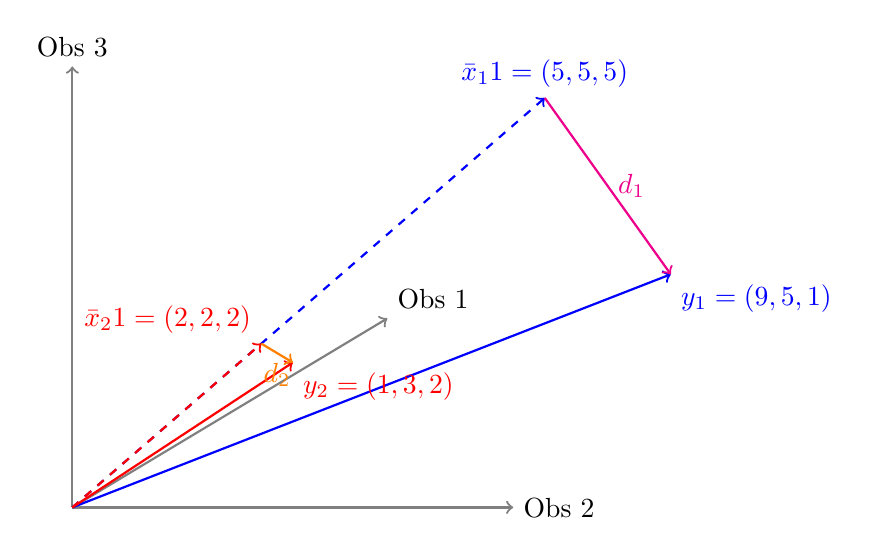
\begin{tikzpicture}[x={(0.5cm, 0.3cm)}, y={(1cm, 0cm)}, z={(0cm, 1cm)}, scale=0.8]
    % Axes
    \draw[->, thick, gray] (0,0,0) -- (10,0,0) node[above right, black] {Obs 1};
    \draw[->, thick, gray] (0,0,0) -- (0,7,0) node[right, black] {Obs 2};
    \draw[->, thick, gray] (0,0,0) -- (0,0,7) node[above, black] {Obs 3};
    
    \draw[->, thick, blue] (0,0,0) -- (9,5,1) node[below right] {$y_1 = (9,5,1)$};
    \draw[->, thick, blue, dashed] (0,0,0) -- (5,5,5) node[above] {$\bar{x}_1 1 = (5,5,5)$};
    \draw[->, thick, magenta] (5,5,5) -- (9,5,1) node[midway, right] {$d_1$};
    
    \draw[->, thick, red] (0,0,0) -- (1,3,2) node[below right] {$y_2 = (1,3,2)$};
    \draw[->, thick, red, dashed] (0,0,0) -- (2,2,2) node[above left] {$\bar{x}_2 1 = (2,2,2)$};
    \draw[->, thick, orange] (2,2,2) -- (1,3,2) node[midway, below] {$d_2$};
\end{tikzpicture}
\end{center}

\vspace{1em}
\noindent \textbf{(c)} Deviation vectors from the origin, lengths, angles, $S_n$, and $R$ \\
Here are the deviation vectors $d_1$ and $d_2$ emanating directly from the origin:
\begin{center}
\begin{tikzpicture}[x={(0.5cm, 0.3cm)}, y={(1cm, 0cm)}, z={(0cm, 1cm)}, scale=1.0]
    % Axes
    \draw[->, gray] (-2,0,0) -- (5,0,0) node[above right, black] {Obs 1};
    \draw[->, gray] (0,-1,0) -- (0,4,0) node[right, black] {Obs 2};
    \draw[->, gray] (0,0,-5) -- (0,0,3) node[above, black] {Obs 3};
    
    \draw[->, thick, magenta] (0,0,0) -- (4,0,-4) node[anchor=north west, fill=white, inner sep=1pt] {$d_1 = (4, 0, -4)$};
    \draw[->, thick, orange] (0,0,0) -- (-1,1,0) node[anchor=south east, fill=white, inner sep=1pt] {$d_2 = (-1, 1, 0)$};
\end{tikzpicture}
\end{center}

Calculate the lengths of the deviation vectors ($L_{d_1}$, $L_{d_2}$):
\[
L_{d_1} = \sqrt{4^2 + 0^2 + (-4)^2} = \sqrt{16 + 0 + 16} = \sqrt{32} = 4\sqrt{2}
\]
\[
L_{d_2} = \sqrt{(-1)^2 + 1^2 + 0^2} = \sqrt{1 + 1 + 0} = \sqrt{2}
\]
Calculate the dot product $d_1 \cdot d_2$:
\[
d_1 \cdot d_2 = (4)(-1) + (0)(1) + (-4)(0) = -4 + 0 + 0 = -4
\]
Calculate the cosine of the angle $\theta$:
\[
\cos(\theta) = \frac{d_1 \cdot d_2}{L_{d_1} L_{d_2}} = \frac{-4}{(\sqrt{32})(\sqrt{2})} = \frac{-4}{\sqrt{64}} = \frac{-4}{8} = -0.5
\]
Relate to $S_n$ (sample covariance matrix with divisor $n=3$):
\[
S_n = \frac{1}{n} \begin{bmatrix} L_{d_1}^2 & d_1 \cdot d_2 \\ d_1 \cdot d_2 & L_{d_2}^2 \end{bmatrix} = \frac{1}{3} \begin{bmatrix} 32 & -4 \\ -4 & 2 \end{bmatrix} = \begin{bmatrix} 32/3 & -4/3 \\ -4/3 & 2/3 \end{bmatrix}
\]
Relate to $R$ (sample correlation matrix). The correlation coefficient $r_{12}$ is exactly $\cos(\theta)$:
\[
R = \begin{bmatrix} 1 & \cos(\theta) \\ \cos(\theta) & 1 \end{bmatrix} = \begin{bmatrix} 1 & -0.5 \\ -0.5 & 1 \end{bmatrix}
\]

\hrulefill

\section*{Problem 3.6}
Given:
\[
X = \begin{bmatrix} -1 & 3 & -2 \\ 2 & 4 & 2 \\ 5 & 2 & 3 \end{bmatrix}
\]

\noindent \textbf{(a)} Matrix of deviations ($X - 1\bar{x}'$) \\
First, find the sample means for each column:
\[
\bar{x}_1 = \frac{-1 + 2 + 5}{3} = \frac{6}{3} = 2
\]
\[
\bar{x}_2 = \frac{3 + 4 + 2}{3} = \frac{9}{3} = 3
\]
\[
\bar{x}_3 = \frac{-2 + 2 + 3}{3} = \frac{3}{3} = 1
\]
Construct the mean matrix $1\bar{x}'$:
\[
1\bar{x}' = \begin{bmatrix} 1 \\ 1 \\ 1 \end{bmatrix} \begin{bmatrix} 2 & 3 & 1 \end{bmatrix} = \begin{bmatrix} 2 & 3 & 1 \\ 2 & 3 & 1 \\ 2 & 3 & 1 \end{bmatrix}
\]
Calculate the deviation matrix $D = X - 1\bar{x}'$:
\[
D = \begin{bmatrix} -1 & 3 & -2 \\ 2 & 4 & 2 \\ 5 & 2 & 3 \end{bmatrix} - \begin{bmatrix} 2 & 3 & 1 \\ 2 & 3 & 1 \\ 2 & 3 & 1 \end{bmatrix} = \begin{bmatrix} -3 & 0 & -3 \\ 0 & 1 & 1 \\ 3 & -1 & 2 \end{bmatrix}
\]
\textbf{Is it full rank?} No. The sum of the columns in a deviation matrix is always zero. Specifically, row 1 plus row 2 plus row 3 equals exactly the zero vector $[0, 0, 0]$. Since the rows are linearly dependent, the rank is at most 2, meaning it is not full rank (rank $< 3$).

\vspace{1em}
\noindent \textbf{(b)} Sample Covariance $S$ and Generalized Variance $|S|$ \\
\[
D'D = \begin{bmatrix} -3 & 0 & 3 \\ 0 & 1 & -1 \\ -3 & 1 & 2 \end{bmatrix} \begin{bmatrix} -3 & 0 & -3 \\ 0 & 1 & 1 \\ 3 & -1 & 2 \end{bmatrix} 
\]
\[
= \begin{bmatrix} (-3)(-3)+(0)(0)+(3)(3) & (-3)(0)+(0)(1)+(3)(-1) & (-3)(-3)+(0)(1)+(3)(2) \\ (0)(-3)+(1)(0)+(-1)(3) & (0)(0)+(1)(1)+(-1)(-1) & (0)(-3)+(1)(1)+(-1)(2) \\ (-3)(-3)+(1)(0)+(2)(3) & (-3)(0)+(1)(1)+(2)(-1) & (-3)(-3)+(1)(1)+(2)(2) \end{bmatrix}
\]
\[
= \begin{bmatrix} 9+0+9 & 0+0-3 & 9+0+6 \\ 0+0-3 & 0+1+1 & 0+1-2 \\ 9+0+6 & 0+1-2 & 9+1+4 \end{bmatrix} = \begin{bmatrix} 18 & -3 & 15 \\ -3 & 2 & -1 \\ 15 & -1 & 14 \end{bmatrix}
\]
Calculate $S = \frac{1}{n-1} D'D = \frac{1}{2} D'D$:
\[
S = \frac{1}{2} \begin{bmatrix} 18 & -3 & 15 \\ -3 & 2 & -1 \\ 15 & -1 & 14 \end{bmatrix} = \begin{bmatrix} 18/2 & -3/2 & 15/2 \\ -3/2 & 2/2 & -1/2 \\ 15/2 & -1/2 & 14/2 \end{bmatrix} = \begin{bmatrix} 9 & -3/2 & 15/2 \\ -3/2 & 1 & -1/2 \\ 15/2 & -1/2 & 7 \end{bmatrix}
\]
\textbf{Generalized Variance $|S|$:} Because the deviation matrix is not full rank, the covariance matrix $S$ is singular. Therefore, $|S| = 0$. \\
\textbf{Geometric Interpretation:} The generalized variance represents the 3D volume formed by the three deviation vectors. Because the vectors are linearly dependent, they lie completely flat on a 2D plane. Since a flat shape has no 3D volume, the generalized variance is zero.

\vspace{1em}
\noindent \textbf{(c)} Total Sample Variance \\
Total variance is the trace of $S$ (sum of diagonal elements):
\[
Tr(S) = s_{11} + s_{22} + s_{33} = 9 + 1 + 7 = 17
\]

\hrulefill

\section*{Problem 3.9}
Given:

\[
X = \begin{bmatrix} 12 & 17 & 29 \\ 18 & 20 & 38 \\ 14 & 16 & 30 \\ 20 & 18 & 38 \\ 16 & 19 & 35 \end{bmatrix}
\]

\noindent \textbf{(a)} Mean corrected matrix $D$ and linear dependence \\
Calculate the column means:
\[
\bar{x}_1 = \frac{12+18+14+20+16}{5} = \frac{80}{5} = 16
\]
\[
\bar{x}_2 = \frac{17+20+16+18+19}{5} = \frac{90}{5} = 18
\]
\[
\bar{x}_3 = \frac{29+38+30+38+35}{5} = \frac{170}{5} = 34
\]
Subtract means to get $D = X - 1\bar{x}'$:
\[
D = \begin{bmatrix} 12-16 & 17-18 & 29-34 \\ 18-16 & 20-18 & 38-34 \\ 14-16 & 16-18 & 30-34 \\ 20-16 & 18-18 & 38-34 \\ 16-16 & 19-18 & 35-34 \end{bmatrix} = \begin{bmatrix} -4 & -1 & -5 \\ 2 & 2 & 4 \\ -2 & -2 & -4 \\ 4 & 0 & 4 \\ 0 & 1 & 1 \end{bmatrix}
\]
The vector establishing linear dependence is $a = \begin{bmatrix} 1 \\ 1 \\ -1 \end{bmatrix}$. Verifying $Da = 0$:
\[
Da = \begin{bmatrix} -4 & -1 & -5 \\ 2 & 2 & 4 \\ -2 & -2 & -4 \\ 4 & 0 & 4 \\ 0 & 1 & 1 \end{bmatrix} \begin{bmatrix} 1 \\ 1 \\ -1 \end{bmatrix} = \begin{bmatrix} -4(1) - 1(1) - 5(-1) \\ 2(1) + 2(1) + 4(-1) \\ -2(1) - 2(1) - 4(-1) \\ 4(1) + 0(1) + 4(-1) \\ 0(1) + 1(1) + 1(-1) \end{bmatrix} = \begin{bmatrix} -5+5 \\ 4-4 \\ -4+4 \\ 4-4 \\ 1-1 \end{bmatrix} = \begin{bmatrix} 0 \\ 0 \\ 0 \\ 0 \\ 0 \end{bmatrix}
\]

\noindent \textbf{(b)} Sample Covariance $S$ and generalized variance \\
Calculate $D'D$:
\[
D'D = \begin{bmatrix} -4 & 2 & -2 & 4 & 0 \\ -1 & 2 & -2 & 0 & 1 \\ -5 & 4 & -4 & 4 & 1 \end{bmatrix} \begin{bmatrix} -4 & -1 & -5 \\ 2 & 2 & 4 \\ -2 & -2 & -4 \\ 4 & 0 & 4 \\ 0 & 1 & 1 \end{bmatrix} = \begin{bmatrix} 40 & 12 & 52 \\ 12 & 10 & 22 \\ 52 & 22 & 74 \end{bmatrix}
\]
Calculate $S = \frac{1}{n-1}D'D = \frac{1}{4}D'D$:
\[
S = \frac{1}{4} \begin{bmatrix} 40 & 12 & 52 \\ 12 & 10 & 22 \\ 52 & 22 & 74 \end{bmatrix} = \begin{bmatrix} 40/4 & 12/4 & 52/4 \\ 12/4 & 10/4 & 22/4 \\ 52/4 & 22/4 & 74/4 \end{bmatrix} = \begin{bmatrix} 10 & 3 & 13 \\ 3 & 5/2 & 11/2 \\ 13 & 11/2 & 37/2 \end{bmatrix}
\]
Because the columns are linearly dependent, the matrix is singular. Thus, $|S| = 0$.
Verify $Sa = 0$:
\[
Sa = \begin{bmatrix} 10 & 3 & 13 \\ 3 & 5/2 & 11/2 \\ 13 & 11/2 & 37/2 \end{bmatrix} \begin{bmatrix} 1 \\ 1 \\ -1 \end{bmatrix} = \begin{bmatrix} 10(1) + 3(1) + 13(-1) \\ 3(1) + 5/2(1) + 11/2(-1) \\ 13(1) + 11/2(1) + 37/2(-1) \end{bmatrix} = \begin{bmatrix} 13-13 \\ 11/2-11/2 \\ 37/2-37/2 \end{bmatrix} = \begin{bmatrix} 0 \\ 0 \\ 0 \end{bmatrix}
\]

\noindent \textbf{(c)} Third column sum verification \\
The relationship $a_1 x_1 + a_2 x_2 + a_3 x_3 = 0$ with $a_1=1, a_2=1, a_3=-1$ yields:
\[
(1)x_1 + (1)x_2 + (-1)x_3 = 0 \implies x_1 + x_2 - x_3 = 0 \implies x_3 = x_1 + x_2
\]
This algebraic equivalence proves the third column is strictly the sum of the first two columns.

\hrulefill

\section*{Problem 3.18}
Given:
\[
\bar{x} = \begin{bmatrix} 0.766 \\ 0.508 \\ 0.438 \\ 0.161 \end{bmatrix}, \quad
S = \begin{bmatrix} 0.856 & 0.635 & 0.173 & 0.096 \\ 0.635 & 0.568 & 0.128 & 0.067 \\ 0.173 & 0.127 & 0.171 & 0.039 \\ 0.096 & 0.067 & 0.039 & 0.043 \end{bmatrix}
\]

\noindent \textbf{(a)} Sample mean and variance of total energy consumption \\
Total consumption is $c'x$ where $c = \begin{bmatrix} 1 & 1 & 1 & 1 \end{bmatrix}'$.
\[
\text{Mean} = c'\bar{x} = 0.766 + 0.508 + 0.438 + 0.161 = 1.873
\]
The variance is $c'Sc$, which equals the sum of all elements in $S$. Calculate row sums first:
\begin{align*}
\text{Row 1 Sum} &= 0.856 + 0.635 + 0.173 + 0.096 = 1.760 \\
\text{Row 2 Sum} &= 0.635 + 0.568 + 0.128 + 0.067 = 1.398 \\
\text{Row 3 Sum} &= 0.173 + 0.127 + 0.171 + 0.039 = 0.510 \\
\text{Row 4 Sum} &= 0.096 + 0.067 + 0.039 + 0.043 = 0.245
\end{align*}
\[
\text{Variance} = 1.760 + 1.398 + 0.510 + 0.245 = 3.913
\]

\noindent \textbf{(b)} Excess of petroleum over natural gas \\
This difference is $b'x$ where $b = \begin{bmatrix} 1 & -1 & 0 & 0 \end{bmatrix}'$.
\[
\text{Mean} = b'\bar{x} = \bar{x}_1 - \bar{x}_2 = 0.766 - 0.508 = 0.258
\]
\[
\text{Variance} = b'Sb = S_{11} - S_{12} - S_{21} + S_{22} = 0.856 - 0.635 - 0.635 + 0.568 = 0.154
\]
The covariance with the total variable from part (a) is $b'Sc$:
\[
Cov(b'x, c'x) = b'Sc = \text{Row 1 Sum} - \text{Row 2 Sum} = 1.760 - 1.398 = 0.362
\]

\hrulefill

\section*{Problem 3.20}
Given the dataset of 25 pairs ($n=25$).

\noindent \textbf{(a)} Calculate via summary statistics \\
First, sum all $x_1$ and $x_2$ values to find means:
\[
\sum x_1 = 292.9 \implies \bar{x}_1 = \frac{292.9}{25} = 11.716
\]
\[
\sum x_2 = 424.4 \implies \bar{x}_2 = \frac{424.4}{25} = 16.976
\]
Calculate sums of squares and cross-products:
\[
\sum x_1^2 = 4315.03, \quad \sum x_2^2 = 9021.70, \quad \sum x_1 x_2 = 4861.90
\]
Determine the sample covariances using $s_{ik} = \frac{\sum x_i x_k - n\bar{x}_i \bar{x}_k}{n-1}$:
\begin{align*}
s_{11} &= \frac{4315.03 - 25(11.716)^2}{24} = \frac{4315.03 - 3431.6164}{24} = \frac{883.4136}{24} = 36.8089 \\
s_{22} &= \frac{9021.70 - 25(16.976)^2}{24} = \frac{9021.70 - 7204.6144}{24} = \frac{1817.0856}{24} = 75.7119 \\
s_{12} &= \frac{4861.90 - 25(11.716)(16.976)}{24} = \frac{4861.90 - 4972.2704}{24} = \frac{-110.3704}{24} = -4.5988
\end{align*}
For the difference $d = x_2 - x_1$, defined by vector $a = \begin{bmatrix} -1 & 1 \end{bmatrix}'$:
\[
\text{Mean} = a'\bar{x} = \bar{x}_2 - \bar{x}_1 = 16.976 - 11.716 = 5.260
\]
Calculate the variance $a'Sa$:
\[
\text{Variance} = s_{11} - 2s_{12} + s_{22} = \frac{883.4136 - 2(-110.3704) + 1817.0856}{24} = \frac{2921.24}{24} = 121.7183
\]

\noindent \textbf{(b)} Calculate from individual differences \\
Sum the individual values $d_j = x_{j2} - x_{j1}$ for all $j=1..25$:
\[
\sum d_j = (13.7 - 12.5) + (16.5 - 14.5) + \dots + (25.6 - 13.0) = 131.5
\]
\[
\text{Mean} = \bar{d} = \frac{131.5}{25} = 5.260
\]
Calculate the sum of squares of these differences:
\[
\sum d_j^2 = (1.2)^2 + (2.0)^2 + \dots + (12.6)^2 = 3612.93
\]
Calculate the variance:
\[
\text{Variance} = \frac{\sum d_j^2 - n(\bar{d})^2}{n-1} = \frac{3612.93 - 25(5.260)^2}{24} = \frac{3612.93 - 691.69}{24} = \frac{2921.24}{24} = 121.7183
\]
\textbf{Comparison:} The results match the summary statistics found in part (a).

\end{document}